\documentclass[../../Aurora C# unofficial manual.tex]{subfiles}

\begin{document}
	\section{Queued ground formation training tasks}
	Original post can be found
	\href{http://aurora2.pentarch.org/index.php?topic=11306.msg131309#msg131309}{here}.
	\\\\
	
	Training Tasks can be queued for ground formations.
	
	Using Create Task when no GFCC is available will add the formation to the queue for the population. Items can be moved up and down the queue, deleted from the queue and renamed while in the queue.
	
	When a GFCC becomes available, the highest queued formation will begin training and an event will be generated. The build cost is not fixed until training begin, so you can change the templates for formations that are still in the queue.
	\begin{figure}[H]
		\centering
		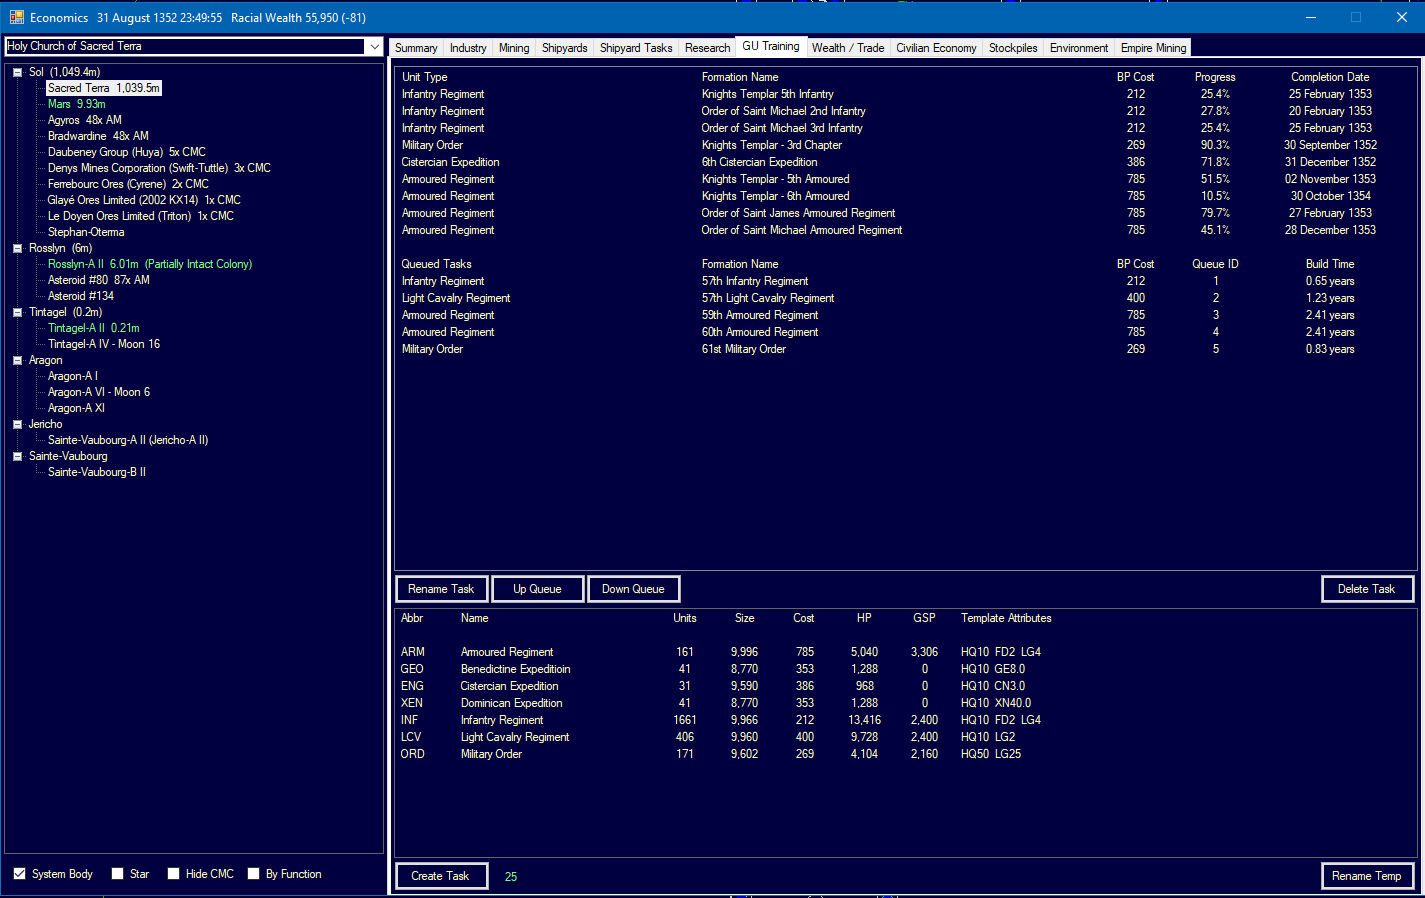
\includegraphics[width=0.95\linewidth]{images/GroundFormationTraining}
		\caption[Ground Formation Training]{Ground Formation Training Example}
		\label{fig:groundformationtraining}
	\end{figure}
\end{document}